% This is samplepaper.tex, a sample chapter demonstrating the
% LLNCS macro package for Springer Computer Science proceedings;
% Version 2.20 of 2017/10/04
%
\documentclass[runningheads]{llncs}
%
\usepackage{graphicx}
% Used for displaying a sample figure. If possible, figure files should
% be included in EPS format.
%
% If you use the hyperref package, please uncomment the following line
% to display URLs in blue roman font according to Springer's eBook style:
% \renewcommand\UrlFont{\color{blue}\rmfamily}
\usepackage{makecell}
\usepackage{tabularx}
\usepackage{multirow}
\usepackage{amsmath}
\usepackage{xcolor}
\usepackage{blkarray, bigstrut}
\usepackage{hyperref}
\hypersetup{colorlinks=true,citecolor=blue}
\usepackage{amsfonts}
\usepackage{dsfont}
\usepackage{lipsum}
\usepackage{adjustbox}
\usepackage{float}
\usepackage{booktabs}
\usepackage{cite}
\usepackage{bm}
\usepackage{pifont}
\newcommand{\cmark}{\ding{51}}%
\newcommand{\xmark}{\ding{55}}%
\newcommand*\rot{\rotatebox{90}}
\newcommand*\OK{\ding{51}}
\begin{document}
%
\title{Supplementary materials}
%
%\titlerunning{Abbreviated paper title}
% If the paper title is too long for the running head, you can set
% an abbreviated paper title here
%
% \author{First Author\inst{1}\orcidID{0000-1111-2222-3333} \and
% Second Author\inst{2,3}\orcidID{1111-2222-3333-4444} \and
% Third Author\inst{3}\orcidID{2222--3333-4444-5555}}
%
% \authorrunning{F. Author et al.}
% % First names are abbreviated in the running head.
% % If there are more than two authors, 'et al.' is used.
% %
% \institute{Princeton University, Princeton NJ 08544, USA \and
% Springer Heidelberg, Tiergarten. 17, 69121 Heidelberg, Germany
% \email{lncs@springer.com}\\
% \url{http://www.springer.com/gp/computer-science/lncs} \and
% ABC Institute, Rupert-Karls-University Heidelberg, Heidelberg, Germany\\
% \email{\{abc,lncs\}@uni-heidelberg.de}}
%
\maketitle              % typeset the header of the contribution
%
%
%
\begin{figure*}[h]
\begin{center}
\centerline{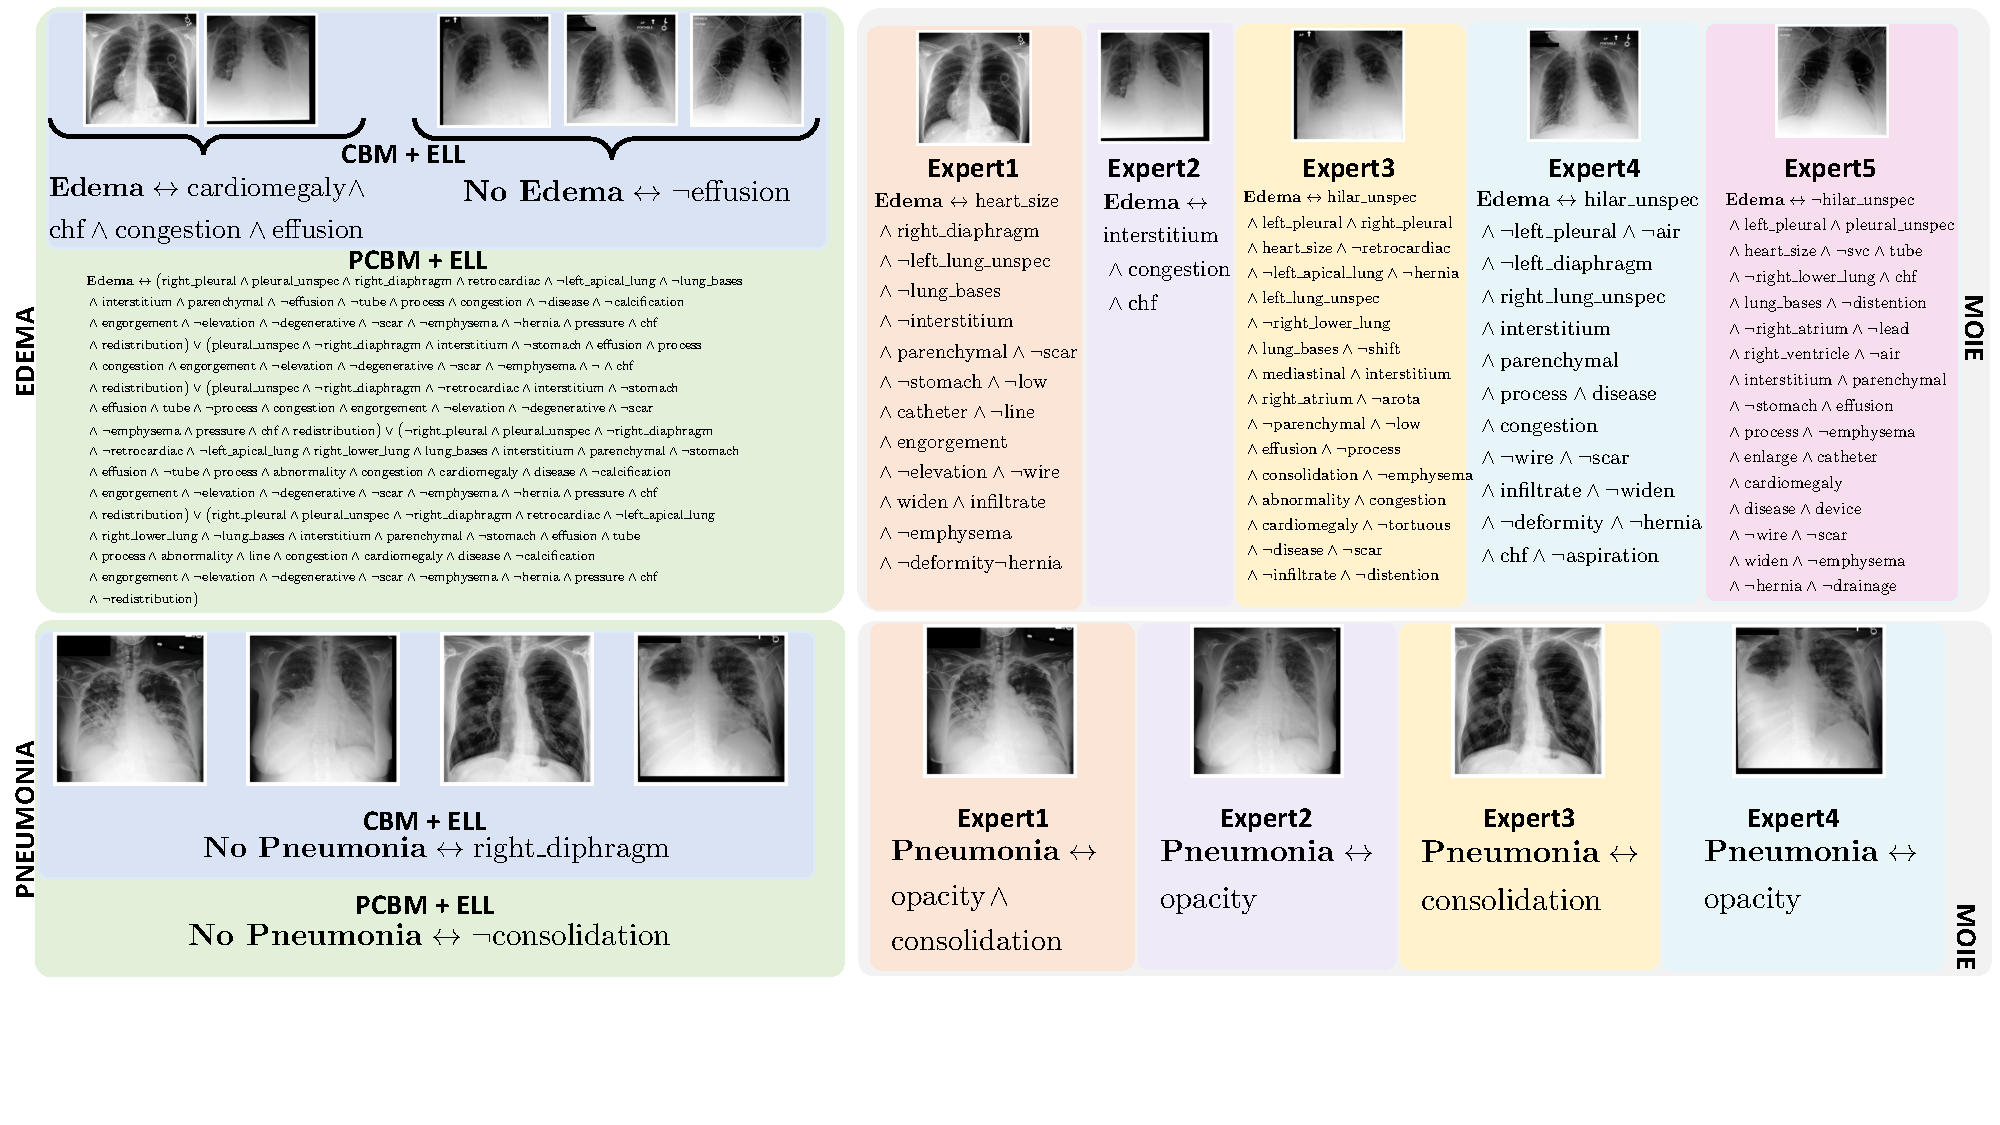
\includegraphics[width=\linewidth]{plots/supp/Supp_qual.pdf}}
\caption{Qualitative comparison of MoIE discovered concepts with the baseline for edema and pneumonia.}
\label{fig:expert_performance_cv_vit}
\end{center}
\end{figure*}

\begin{figure*}[h]
\begin{center}
\centerline{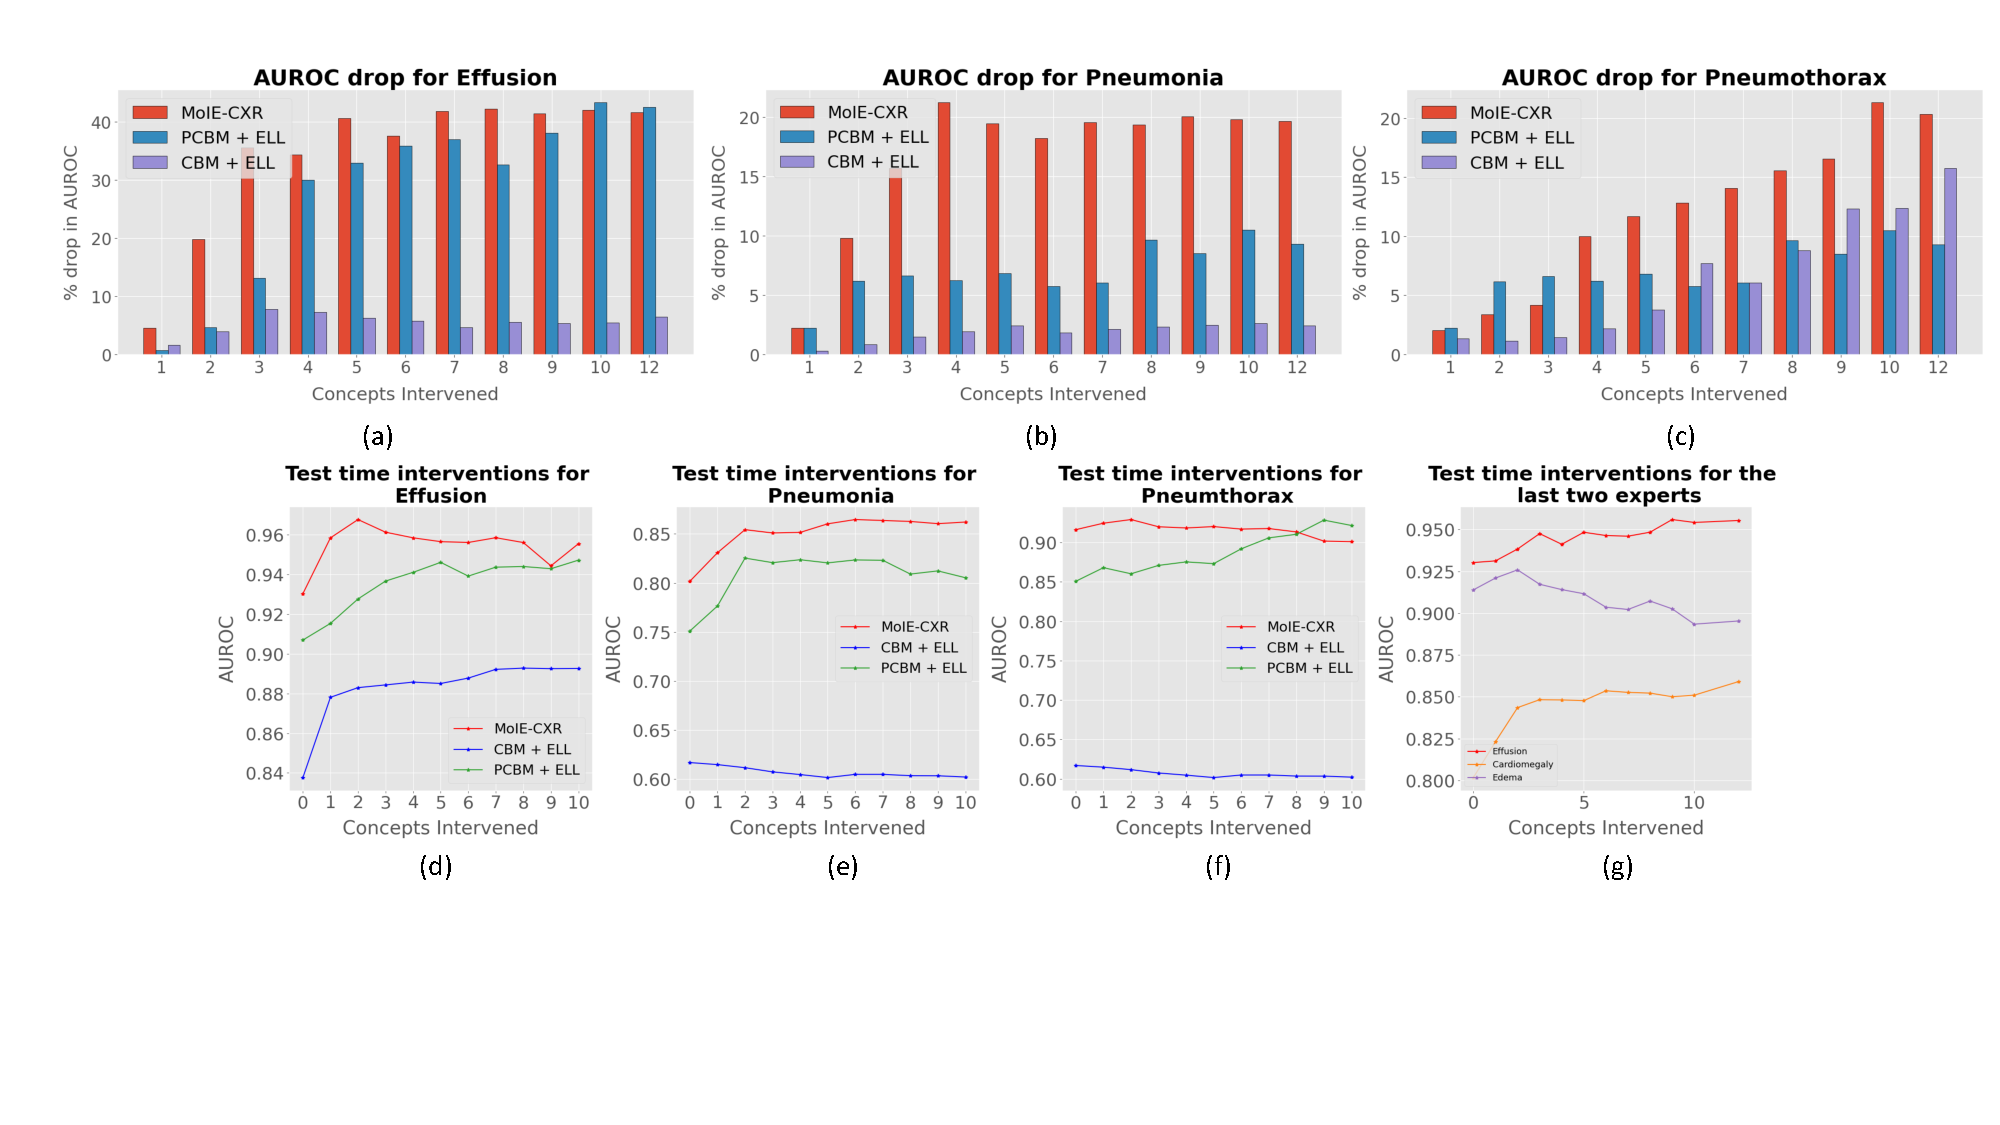
\includegraphics[width=\linewidth]{plots/supp/Supp_Quant_concepts.pdf}}
\caption{\textbf{(a-c):} Performance drop after zeroing out the concepts iteratively. The drop indicates the concepts to be more significant for prediction. \textbf{(d-g):} Test time interventions of concepts considering the ground truth concepts as an oracle on all samples (d-f), on the ``hard'' samples (g), covered by only the last two experts of MoIE-CXR.}
\label{fig:expert_performance_cv_vit}
\end{center}
\end{figure*}

\begin{figure*}[h]
\begin{center}
\centerline{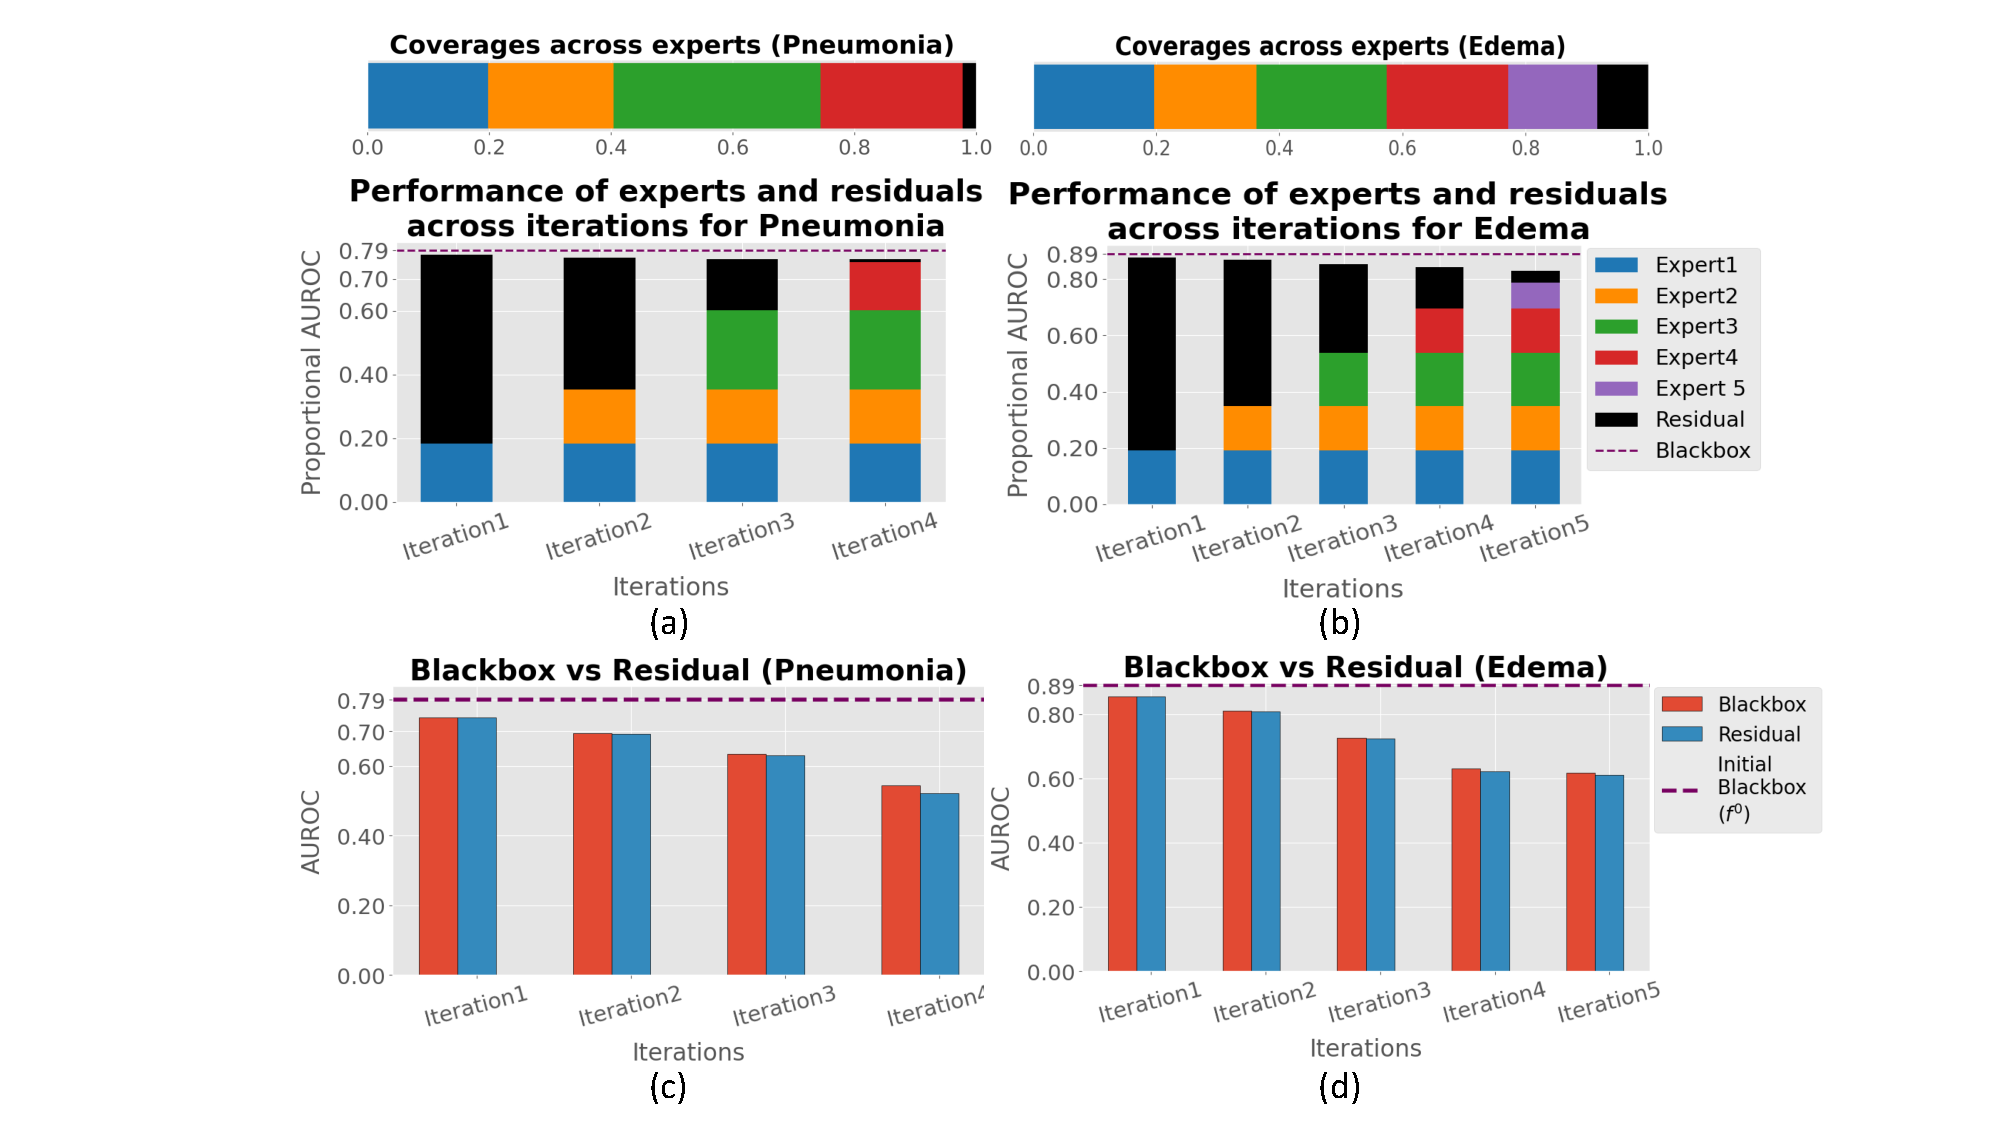
\includegraphics[width=\linewidth]{plots/supp/Supp_Experts.pdf}}
\caption{\textbf{(a-b)}: The performances of experts and residuals across iterations for pneumonia and edema. \textbf{(c-d)}: Performance comparison of the residuals and $f^0$ for the samples covered by the successive residuals.
}
\label{fig:expert_performance_cv_vit}
\end{center}
\end{figure*}

\begin{table}[H]
\caption{Hyperparameters of interpretable experts ($g$) for the dataset MIMIC-CXR.}
\label{tab:g_config_mimic_cxr}
\begin{center}
\begin{tabular}{l c c c c c }
\toprule 
    \thead{\textbf{Hyperparameter}} & 
    \thead{\textbf{Effusion}} & 
    \thead{\textbf{Cardiomegaly}} & 
    \thead{\textbf{Pneumothorax}} &
    \thead{\textbf{Pneumonia}} &
    \thead{\textbf{Edema}} \\
  
\midrule 
       Batch size & 1028 & 1028 & 1028 & 1028 & 1028   \\
       Learning rate & 0.01 & 0.01 & 0.01 & 0.01 & 0.01\\
       $\lambda_{lens}$ & 0.0001 & 0.0001 & 0.0001  & 0.0001 & 0.0001\\
       $\alpha_{KD}$ & 0.99 & 0.99 & 0.99 & 0.99 & 0.99 \\
       $T_{KD}$ & 20 & 20 & 20  & 20 & 20  \\
       hidden neurons & 30, 30 & 20, 20 & 20, 20 & 20, 20 & 20, 20 \\
       $\lambda_s$ & 96 & 1024 & 256 & 256 & 128   \\
       E-Lens ($T_{lens}$) & 7.6 & 7.6 & 10 & 10 & 7.6\\
       \# Expers ($T_{lens}$) & 5 & 4 & 5 & 4 & 5\\
\bottomrule
\end{tabular}
\end{center}
\end{table}

% \begin{table}[H]
% \caption{Hyperparameter setting of interpretable experts ($g$) for the dataset MIMIC-CXR}
% \label{tab:g_config_mimic_cxr}
% \begin{center}
% \begin{tabular}{l c c c c c }
% \toprule 
%     \thead{\textbf{Hyperparameter}} & 
%     \thead{\textbf{Effusion}} & 
%     \thead{\textbf{Cardiomegaly}} & 
%     \thead{\textbf{Pneumothorax}} &
%     \thead{\textbf{Pneumonia}} &
%     \thead{\textbf{Edema}} \\
  
% \midrule 
%        Batch size & 1028 & 1028 & 1028 & 1028 & 1028   \\
%        Learning rate & 0.01 & 0.01 & 0.01 & 0.01 & 0.01\\
%        $\lambda_{lens}$ & 0.0001 & 0.0001 & 0.0001  & 0.0001 & 0.0001\\

% \bottomrule
% \end{tabular}
% \end{center}
% \end{table}



% \bibliographystyle{splncs04}
% \bibliography{main}
\end{document}
